\chapter{Introducción}
% Esta sección es en su mayoría lo que ya esta en el protocolo
% por lo que si se van a hacer correcciones en el protocolo hay mantener esta sección y el protocolo con la información más reciente.
% Las secciones que en teoria aparecen aqui son:
% \begin{itemize}
%     \item Resumen
%     \item Palabras clave
%     \item Antecedentes
%     \item Justificación
%     \item Planteamiento del problema
%     \item Objetivos
%     \item Estado del arte
%     \item Descripción del documento
% \end{itemize}

%{palabras clave, planteamiento del problema[incluye: antecedentes, justificación], objetivos, estado del arte, propuesta}

%\begin{itemize}
%    \item Palabras Clave
%    \item Planteamiento del problema
%    \item Objetivos
%    \item Estado del arte
%    \item Descripción del documento
%\end{itemize}


LaTeX es un sistema de tipografía de alta calidad que incluye características útiles para el diseño de documentos técnicos y científicos. Este software, es de facto un estándar para la comunicación y la publicación de artículos científicos. %\cite{Agregar Citas}.
\bigskip

A pesar de lo práctico que puede ser LaTeX, si el documento contiene muchas expresiones matemáticas, puede resultar tedioso para el usuario escribir dichas expresiones. Por lo que este Trabajo Terminal tiene como finalidad brindar una herramienta que permita amenizar la interacción de nuevos usuarios al escribir expresiones matemáticas en LaTeX mediante el uso de una aplicación móvil y una aplicación web, esta última capaz de reconocer expresiones matemáticas en imágenes que pueden ser tomadas desde el mismo \texttt{smartphone}.
\bigskip


\section{Palabras Clave}
[Aplicación móvil, LaTeX, Image Captioning] %siento que faltan
\section{Planteamiento del problema}

%\textbf{JUSTIFICACIÓN}

 Debido a la naturaleza de LaTex (producción de documentos de alta calidad) los usuarios que en su mayoría utilizan este sistema pertenecen a la comunidad científica y académica y específicamente provenientes de áreas como las ciencias de la computación, física y matemáticas para producción de documentos en su mayoría de divulgación de conocimiento, sin embargo de acuerdo a diversos estudios \cite{latexUsage} que muestran que en áreas de ciencia como Medicina, Psicología, GeoCiencias entre otras, el uso de LaTex no es tan extendido como se puede ver en la Figura \ref{fig:estadisticasUso}, impidiendo que estos usuarios aprovechen las ventajas que un sistema como LaTex ofrece, esto debido a que requiere que los usuarios estén familiarizados con procesos específicos como la compilación de código y por lo tanto para aquellos usuarios que no tienen relación directa con estos procesos el superar la curva de aprendizaje puede llegar a ser complicado y en muchos casos llegan a optar por utilizar alternativas que no impliquen los procesos ya mencionados que no proporcionan la calidad que LaTex puede llegar a ofrecer.
\\\\%\bigskip

\begin{figure}
	\centering
	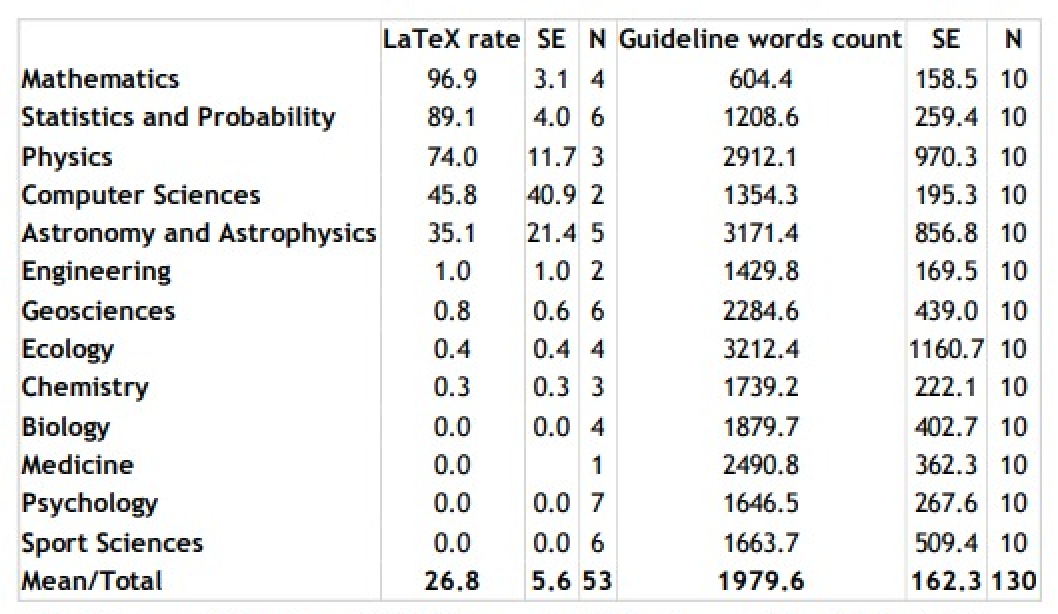
\includegraphics[width=0.8\textwidth]{capitulo1/images/estadisticasUso.png}
	\caption{Resumen de estadisticas del uso de LaTeX en disciplinas de ciencia (\% de papers enviados) y el número de palabras contenidas en los lineamientos para los autores.}
	\label{fig:estadisticasUso}
\end{figure}

El enfoque del presente trabajo terminal consiste en desarrollar un sistema conformado por una aplicación tanto móvil como web que en conjunto permitan tomar fotografías y extraer las expresiones matemáticas para su posterior traducción con el objetivo de introducir a nuevos usuarios de cualquier área de estudio al sistema LaTex y así superar esa curva de aprendizaje en un menor tiempo y de inicio ser una herramienta práctica, si bien es cierto (como se puede ver en la tabla																							 \ref{tab:state_of_art}) existen otros sistemas que buscan resolver el problema de traducir expresiones matemáticas a partir de imágenes, sin embargo, ninguno de ellos ataca este problema directamente y ninguno de estos cuenta con una aplicación móvil para resolver dicho problema.
\\\\%\bigskip

Con el desarrollo de este prototipo de sistema se debe tener en cuenta que específicamente se ataca el problema de expresiones matemáticas (que a diferencia del reconocimiento de texto plano el cual es un problema que se considera resuelto por los buenos resultados que se han obtenido) este sigue siendo un problema abierto debido a su naturaleza jerárquica y bidimensional y que en la actualidad las soluciones existentes no brindan buenos resultados aún \cite{chino}, por lo que mejorar los resultados del estado del arte no es el objetivo de este trabajo.
%\\\\%\bigskip
%El tiempo estimado de desarrollo del Trabajo Terminal es de diez meses, empezando en el mes de agosto 2019 y concluyendo en el mes de mayo del 2020 


\newpage

\section{Estado del arte}

%ESTADO DEL ARTE
Algunos sistemas similares que se han desarrollado son:
\begin{itemize}
	\item Mathphix \cite{mathphix}%
	\item MyScript Nebo \cite{nebo}%[Cita].
	\item SESHAT \cite{AlvaroPR16}%[4].
	\item IDEAL Math Writer \cite{idmath} %[5].
\end{itemize}
Los cuales se describen en la tabla \ref{tab:state_of_art}: \\\\
\begin{longtabu} to 1\textwidth { | X[m,c] | X[m,c] | X[m,c] | }
	\hline
	\textbf{SOFTWARE} & \textbf{CARACTERISTICAS} & \textbf{PRECIO EN EL MERCADO} \\
	\hline
	Mathpix  & Es una aplicación de escritorio en la que puedes usar un comando para tomar una captura de pantalla y convertir el texto capturado a LaTeX. También cuenta con un API de pago  & Este producto cuenta con diferentes planes de pago según su uso o el tiempo que decidas pagarlo. Tiene distinto trato para empresas. Un ejemplo de suscripción mensual es \$99 dólares el mes.  \\
	\hline
	MyScript Nebo  & Es una aplicación Android que transforma el texto escrito en el dispositivo en texto digital. Incluye soporte para ecuaciones. Es necesario el uso de una pluma digital.& \$189.00 en Google Play Store  \\
	\hline
	Mathpix  & Es una aplicación de escritorio en la que puedes usar un comando para tomar una captura de pantalla y convertir el texto capturado a LaTeX. También cuenta con un API de pago  & Este producto cuenta con diferentes planes de pago según su uso o el tiempo que decidas pagarlo. Tiene distinto trato para empresas. Un ejemplo de suscripción mensual es \$99 dólares el mes.  \\
	\hline
	SESHAT  & Es un proyecto de doctorado de la Universidad Politécnica de Valencia open source. Convierte el texto de imágenes en texto digital y en formato LaTeX. Soporta ecuaciones. Necesita ser instalado mediante terminal en Linux. & No es una aplicación comercial  \\
	\hline
	\caption{Resumen de productos similares}
	\label{tab:state_of_art}
\end{longtabu}


\section{Objetivos}
%\textbf{OBJETIVO}
Desarrollar un sistema que reconozca un conjunto delimitado de tipos de expresiones matemáticas en una imagen dada y las traduzca a un formato que un compilador de LaTeX pueda procesar.
\subsection{Objetivos específicos}
\begin{enumerate}
	\item Desarrollar una aplicación móvil que permita tomar fotografías y que pueda conectarse a una aplicación web para su posterior procesamiento.
	\item Desarrollar un módulo de análisis de imágenes para el reconocimiento de las expresiones matemáticas.
	\item Desarrollar un módulo de traducción a LaTeX.
	\item Desarrollar la interfaz que conecte el módulo de análisis de imágenes alojado en el servidor con la aplicación móvil y web.
\end{enumerate}


\section{Resultados esperados}
Podemos separar el sistema en dos bloques principales, el primero el lado del cliente el cual se compondrá de la aplicación móvil y de la interfaz web con las cuales el usuario podrá interactuar. Por otro lado, se tiene la parte del servidor web que se conectará con la aplicación móvil, en el servidor se encontrará la parte de análisis de imágenes junto con el módulo de traducción. Finalmente se tiene el módulo de gestión de usuarios. Esto se puede apreciar en la Figura \ref{fig:arquitectura}.%ref %%AYUDA, NO ESTA REFERENCIANDO

El sistema se compone de cinco módulos:
\begin{enumerate}
    \item Módulo de análisis de imágenes. Este módulo se encargará de procesar las imágenes e identificar un conjunto delimitado de tipos de expresiones matemáticas.
    \item Módulo de traducción. Este módulo tomará como entrada lo obtenido en la etapa de análisis de imágenes y regresará el respectivo código de LaTeX que represente las expresiones matemáticas reconocidas.
    
    \item Módulo de gestión de usuarios. En este módulo se hará la gestión de la información de los usuarios de la aplicación, lo que implica tener un control de su información y de los archivos que generen al usar el sistema. Esta gestión de usuarios estará presente tanto en la aplicación móvil como en el servidor web.

    \item Aplicación móvil. Este módulo consiste en el desarrollo de la aplicación móvil que el usuario final llevará en su Smartphone y con la cual podrá tomar fotos que cumplan ciertos requisitos para así obtener el código en LaTeX a través de la comunicación con la aplicación web.

    \item Servidor web. El servidor web hará uso de los módulos de análisis de imágenes, de traducción y de gestión de usuarios por lo que deberá de mantener una comunicación entre ellos y la aplicación móvil, así como con la base de datos. Además, es el punto que permite visualizar el resultado final de todo el procesamiento de imágenes a través de una interfaz web.
\end{enumerate}
Los productos esperados del Trabajo Terminal son:
\begin{enumerate}
    \setcounter{enumi}{5}
    \item Código fuente del trabajo desarrollado (todos los módulos).
    \item Documentación técnica del sistema.
\end{enumerate}

\begin{figure}[h]
\centering
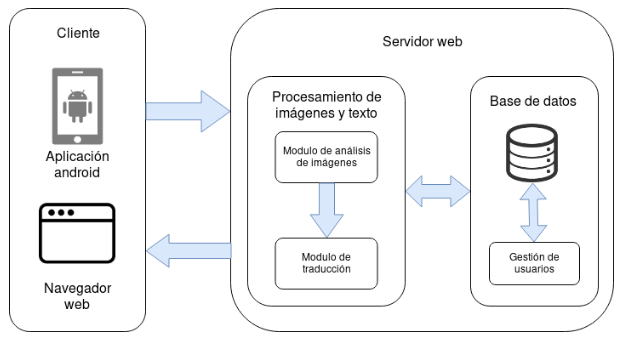
\includegraphics[width=1.0\textwidth]{capitulo1/images/arquitectura.png}
\caption{Arquitectura del sistema.}
\label{fig:arquitectura}
\end{figure}
\newpage

\section{Metodología} Para el desarrollo del proyecto se eligió la metodología incremental debido a que permite dividir el proyecto en pequeñas iteraciones secuenciales \cite{iterativeDevelopment}. En cada iteración, se tendrá la libertad de implementar los requerimientos más apropiados para un correcto flujo en el desarrollo de la aplicación. A pesar de que la metodología por incrementos permite flexibilidad para modificar los requerimientos funcionales, se tienen planeadas las siguientes actividades que se llevarán a cabo en distintas iteraciones:
\bigskip
\begin{itemize}
    \item Se realizará obtención de requerimientos, el análisis y diseño (modelado) del módulo de análisis de imágenes, construcción del módulo y finalmente se harán pruebas sobre este.
    \item El módulo de traducción se realizará paralelamente al módulo anterior, al tener esto listo y con sus respectivas validaciones aprobadas se realizará el desarrollo y con ello realizar pruebas sobre todos los componentes que se tengan hasta este punto.
    \item Se desarrollará la aplicación móvil la cual su principal funcionalidad es la obtención de las imágenes y su comunicación con el servidor web.
    \item Se desarrollará el módulo de servidor web ya que es lo que nos servirá para conectar el módulo de análisis de imágenes con la aplicación móvil y se probará la comunicación entre cada uno de estos elementos.
\end{itemize}




%----------------------------OBJETIVOS

\newpage


% Ya hay muchos trabajando en este tema utilizando redes neuronales, lo interesante del nuestro es ponerlo en una aplicación web/android 

% En el entrenamiento se pueden probar varias funciones de cada capa de la arquitectura. 

% Wandb logro un resultado mejor que el del estado del arte, es decir, mejor que el articulo de harvard 

% Los resultados son buenos con imagenes preprocesadas del conjunto de entrenamiento, en imagenes que se esperan de usuarios no es tan bueno el resultado. 

% ¿El estado del arte ataca ecuaciones a mano o solo screenshots? Esto es importante a considerar si nos basamos en estos trabajos para el nuestro. 

% El preprocesamiento de la imagen se puede atacar con dos posibles formas, esto puede ser la parte de nuestro TT que sea la innovadora 

% El preprocesamiento de la imagen nos va a matar con Benoso. 

% Una amenaza es wandb entre otros investigadores igual es importante tomarlo en cuenta para la factibilidad ya que en cualquier momento pueden surgir nuevos avances y dejarnos obsoletos 

% Quiubole con que si utilizan un latex parser para la normalizacion 

% No manches hay muchos trabajos al respecto de gente pro =( 

% Hay un chingo de terminos que no entiendo 

% Todo lo hacen con un conjunto de entrenamiento ya preprocesado nada de input de usuario 